% see https://www.usenix.org/sites/default/files/template.la_.txt for original.
\documentclass[letterpaper,twocolumn,10pt]{article}
\usepackage{usenix,epsfig,endnotes}
\begin{document}

%don't want date printed
\date{}

%make title bold and 14 pt font (Latex default is non-bold, 16 pt)
\title{\Large \bf Federated Consistency for User-Centric Distributed Data Storage}

%for single author (just remove % characters)
\author{
{\rm Benjamin Bengfort}\\
University of Maryland\\
bengfort@cs.umd.edu
\and
{\rm Pete Keleher}\\
University of Maryland\\
keleher@cs.umd.edu
} % end author

\maketitle

% Use the following at camera-ready time to suppress page numbers.
% Comment it out when you first submit the paper for review.
% \thispagestyle{empty}


\subsection*{Abstract}

Federated consistency refers to a property of distributed systems wherein individual replicas maintain variable consistency levels. By allowing replicas to manage local storage independently of the system as a whole, a distributed storage system can take advantage of the high availability of eventually consistent systems while simultaneously providing strong guarantees about durability and ordering through a backbone consensus group. Unlike a homogenous, low latency data center, we believe that federated consistency enables heterogenous, variable latency, partition prone distributed storages such as those in personal clouds or in environments where backbone infrastructure has been lost and will perform better than centralized, high latency cloud storage.

\section{Introduction}

% I hate this paragraph: if we lead with the CAP theorem then no one will take the paper seriously. Particularly because of HAT and Brewer's article.

Distributed storage systems provide durability and availability by replicating data across multiple nodes, increasing redundancy and processor locality. These systems are described as a collective whole of independent, local nodes who share information over a potentially unstable or untimely network. As a result, most discussions concerning these types of systems focus on whether or not a node's view of the data is correct (consistency), whether or not clients can make progress (availability), and how the system repairs itself in the event of failure (partition tolerance).

Because of this characterization, the discussion of distributed storage systems is highly dependent on the network environment and distributed topology; and as a result, recent literature has shifted focus from networked file systems to cloud storages residing in data centers. In this environment, partitions are generally caused by wide area network failure, nodes are homogenous with similar capabilities, and intra-node network latency is minuscule relative to the client's connection. In such an environment, it is possible to reason about the trade-off between consistency and latency using a metric such as probabilistically bounded staleness \cite{bailis_quantifying_2014} and to explore a variety of consistency and transaction protocols from timing certainty using GPS and atomic clocks \cite{corbett_spanner_2013} to highly available key-value stores \cite{decandia_dynamo_2007}.

% Am I allowed to cite Dropbox?

By encapsulating these systems in a data center environment, performance measurements omit or treat as constant the bulk of latency encountered in real usage: the request latency from a user to the cloud and back again. In a user-oriented distributed data store such as Dropbox which syncs files across devices through a centralized cloud store it has been observed that frequent, short updates to user data causes inefficient traffic between the user's replicas and Dropbox \cite{li_efficient_2013} and that session acquisition is the primary bottleneck in synchronization performance \cite{drago_inside_2012}. Both of these studies propose a local middleware to alleviate these problems, but we take a stronger view: user devices should not simply be clients of web services that provide replication, they should be active participants acting as replicas themselves.

This forces us to have a new view of how systems behave. User devices have a variety of requirements and limitations from capacity to performance, and not all devices can perform leadership or relay roles. The distributed network is more partition prone as user devices are not always on or connected and mobility means highly variable latencies. Users switch devices, collaborate, and have preferences about what applications see what data and when. As a result, no single consistency, availability, or convergence mechanism can be directly applied.

In this paper we propose a vision for \textit{federated consistency}, an envelope term for a scheme where flexible consistency policies are mixed, modified, and coordinated to provide application-specific availability in user local networks. We present a base architecture for a distributed storage system that can utilize federated consistency but still provide strong guarantees, then discuss the consistency and consensus algorithms that might be implemented and how they interact. Finally, we propose a mechanism for evaluating the performance of such a system and highlight future work in this topic.

\subsection{Distributed Environment}

We assert that the computing and network environment of a distributed system plays a large role in determining not just the performance of the system, but in fact its behavior. A simple example is the election timeout parameter of the Raft consensus protocol, which must be significantly greater than the average time to broadcast and receive responses, and significantly less than the mean time between failure \cite{ongaro_search_2014}. If this requirement is not met, then the system will not be able to maintain a leader who will be displaced before heartbeat messages arrive or it will be unable to quickly recover when the leader fails or is cut off from the quorum. As a result, the relationship of timeouts is critically dependent on the mean latency ($\lambda_{\mu}$) of the network. Extended studies on Raft propose heuristics such as $T = \lambda_{\mu} + 2\lambda_{\sigma}$ to determine timeouts based on the distribution of observed latencies, then setup the heartbeat as $\frac {T} {2}$ and an election timeout as the interval $U(T,2T)$ \cite{howard_raft_2015}. Real world systems such as etcd, a distributed key-value store by CoreOS, use a ``tick'' measure instead of milliseconds, which is computed in real time based on real performance; etcd recommends a 10:1 ratio of ticks for election timeouts to heartbeat messages \cite{mizerany_etcd_2016}.

% What about anti-entropy delays or other mechanisms?

Heuristics, distribution analysis, and modeling of the underlying distributed environment to determine system behavior are only effective when the environment exhibits a regular distribution of failure or latency. Such distributions are guaranteed in a data center where the environment is well managed and controlled. Most devices in a data center have similar specifications and are utilized for a similar suite of applications (servers or services that respond to requests). They are connected by high performance, low latency networks organized by switches in racks. These devices are always on, do not move, and have a number of amenities such as back up power and redundant disks.

In contrast, smaller scale, user-centric networks consist of fewer, application-specific devices that range from mobile devices to workstations. These devices connect to a variety of networks, from limited bandwidth cellular connections to high speed broadband links. A complete view of all devices for a single user will have irregular communication topologies based on location, e.g. a home network vs a work network, with mobile devices that can connect to both. Partitions can also easily occur when devices are powered off or leave the range of a network connection, and must be considered routine. Because a variety of applications with different data requirements or use cases are run on each device, a single consistency model (or view of the data) is not applicable. Moreover, the different specifications of each device mean that not all devices can equally participate in a distributed storage system (store a complete replica, participate as a leader, or act as a relay).

In order to reason about how a distributed system performs in a user centric context, we propose a model of the computing and network environment that has the following properties:

\begin{enumerate}
    \item \textbf{Heterogeneous devices}: there is a range in the performance and capacity of devices in the network, particularly in terms of storage capacity and the amount of time required to process and respond to messages.
    \item \textbf{Highly variable latencies}: network connections have a wide range of possible latencies, and the latency distribution also varies over time (for example as mobile devices move between networks).
    \item \textbf{Partition prone networks}: nodes become unreachable on a routine basis, and can rejoin the network at any time.
    \item \textbf{Irregular topologies}: not all nodes are connected at all times and moreover the topology is dynamic and connections can be added or removed.
\end{enumerate}

We believe that the challenge this environment poses to a distributed storage system will lead to valuable research both to address how consistency models that already exist operate in these environments as well as new protocols that increase performance or resilience. We also take the view that studying the more difficult case of these types of networks will also inform how more consistent environments behave.

\subsection{Requirements}

As the environment of distributed systems plays a large role in determining their behavior, so to does the specification or application of the system. Generally speaking the literature usually refers to file systems when discussing user centric distributed storage, and database systems for cloud storage, though the difference between the two can easily be blurred by representing a file system as a key-value store such as is done in the Amazon Simple Storage Service (S3) \cite{bermbach_eventual_2011}.

For the purposes of discussing federated consistency, we will generalize the requirements of the distributed system as follows. The system must manage multiple, independent objects whose data structure is defined solely within the context of the object (e.g. the system can be a simple key-value store, a relational database, or a file system). A single view of the system is given by a single user, and that view must be consistent with respect to the user's application. However, a system can maintain multiple views with multiple users interacting with the same objects (collaborative transactions).

% Citation for bursty workloads?

Both in single and multi user contexts, the workload is variable with bursty accesses, unlike cloud storages which experience near constant workloads. This burstiness comes not only from routine work schedules but also because users typically don't access multiple devices simultaneously. Whereas many consistency models are designed for high availability through load balancing, the availability concerns in a user-centric distributed system tend to be application-specific. For example, photography workloads tend to be single writes (at the time of the photograph) but require multiple sequential reads as rapidly as possible. On the other hand, collaborative document editing requires linearizable, rapid writes along with read your write semantics.

% Citations for the flattening stuff?

The required guarantees for the system also are application specific. For the most part, durability is a constant and data loss is a bad thing. However, not all versions or temporary files need to be stored. Generally speaking more recent versions should remain durable, while historical versions can removed in a process called \textit{temporal aspect flattening}. Complete replication is also typically not a requirement, some devices require partial replication due to storage constraints, while others require only file formats specific to the application. Deciding what is stored on a partial replica is described as \textit{spatial aspect flattening}.  Finally, the rate at which objects are replicated is bound by the available bandwidth, some applications like video streaming should not share bandwidth through a replication process. Decisions about when and how replication occurs is referred to as \textit{synchronization aspect flattening}.

These requirements can be summarized as follows:

% Convert to a table
\begin{itemize}
    \item Management of multiple objects
    \item User centric views and multiple users
    \item Variable, bursty workloads
    \item Limited capacity and durability
    \item Partial replication
    \item Fair or limited resource use
    \item Multiple replicas and local replication
\end{itemize}

The last requirement dovetails with the irregular topologies discussed in the previous section. As the number of users in a distributed system increases, so do the number of replicas and partial replicas. Many consistency policies do not scale linearly therefore federated consistency needs to consider localities and partial quorums that emerge to global distributed semantics and guarantees.

\subsection{Examples}

We conclude the motivating section with three examples of distributed systems that might benefit from federated consistency: a personal cloud, disaster recovery/search and rescue, and highly mobile sensors.

\textbf{Personal Clouds} are a twist on distributed file systems that attempt to integrate storage across a wide area network and optionally with cloud storage. Personal clouds leverage mobile devices and high bandwidth connections to provide reliable replication. The primary advantage of a personal cloud is the low latency local network connections and the fact that synchronization to other devices does not require two round trips from a remote replica and back. Personal clouds put data ownership and management back into the user's hands who can better manage personal security and encryption as well as cost.

Single user personal clouds can be adapted into multiple user clouds with boundary-specific replication of shared objects. A hierarchical approach means that users can participate in multiple clouds or construct medium to large distributed storages. Collaboration and shared editing benefits from the same advantages, namely local network latency as opposed to multiple round trips to centralized application servers.

\textbf{Search and Rescue} networks are deployed in areas with no backbone connection either due to the remoteness of the activity or service interruptions after a disaster. As a result, these systems typically use mesh networking to create a local connectivity fabric, often in a hierarchical fashion. For example, in a large-scale disaster such as a hurricane, fire trucks may contain primary bandwidth links via satellite or point-to-point broadband connections, police squad cars may provide additional range by relaying wireless connections, and individual first responders may carry a variety of sensors and communication equipment. Remote units relay status information back to the primary bandwidth links, which in turn connect to a central operations command.

Due to the limited resources in such an environment and varying level of message priorities, multiple consistency levels are required. Routine updates with position information can be eventually consistent within some quality of service guarantee, however, alerts or triage information must arrive in a timely and correct fashion. Non-real-time data needs to be durable and ordered so that post operation analysis such as conducting structural audits or directing repair logistics is correct and verifiable.

\textbf{Highly Mobile Sensors} take advantage of new platforms such as robotic or arial vehicles to deploy a variety of sensors including audio and video to locations on demand. These sensors networks can be very large, such as video surveillance or photography (for example filmography recording a cycling race) or smaller and highly connective as in triage sensors in a hospital emergency room. Similar to search and rescue applications, these systems may have variable network connectivity or use mesh networking; however it is their mobility that is the key factor requiring federated consistency. Mobile sensors create irregular, dynamic topologies that require local consistency guarantees. Many strong consistency models require three phase commit for membership changes; but in a mobile sensor network, membership changes can be the norm not the exception. Federated consistency allows this type of distributed system to adapt as the topology adapts.

\section{Consistency Levels}

A federated consistency approach utilizes policies regarding temporal, spatial, and synchronization aspects to determine the behavior of a replica with regards to a set of objects. Consistency levels in such a system can be characterized on the range from eventually consistent to causal consistency to sequential consistency. This consistency range is also specified as the range between weak consistency (no node in the system is guaranteed to have the most up to date version) to strong consistency (all accesses view a single, consistent state).

\subsection{Eventual Consistency}

Eventual consistency is typically described using Werner Vogels' now popular definition: ``if no new updates are made to an object, eventually all accesses will return the last updated value'' \cite{vogels_eventually_2009}. This model offers liveness and availability to clients by simply returning the latest observed value of the object, however it is subject to staleness, in that the replica may be operating on old (stale) objects, though it can be shown that the extent of the staleness is bounded by the mean latency of the distributed system \cite{bailis_quantifying_2014,bailis_probabilistically_2012}.

Eventually consistent systems trade reduced response times for what is essentially a last-writer wins approach to data storage, which can have significant consequences for application behavior. Careful application design such as the use of commutative or associative operations on conflict-free replicated data types (CRDTs) \cite{shapiro_conflict-free_2011} or the careful application of immutable objects \cite{helland_immutability_2015} can mitigate some of the effects of this trade off. Other models such as Scatter employ multiple levels of consistency within the eventually consistent context, such as fully linearizable storage for a single key, but no linearization of multi-key transactions \cite{glendenning_scalable_2011}.

The implementation of eventually consistent systems utilizes anti-entropy \cite{demers_epidemic_1987} mechanisms to perform pairwise replication between two replica servers and to recover from partitions. For example, Bayou allows clients to perform file accesses locally then uses \cite{terry_managing_1995,terry_session_1994} anti-entropy sessions to propagate writes while also resolving conflicts through a policy based session guarantees. Bayou allows liveness, minimizes network usage, and delegates conflict handling to the application layer. Anti-entropy is introduced via gossip protocols (also called rumor mongering) where nodes spread rumors by randomly contacting a local neighbor and updating them. Gossip protocols solve the local broadcast problem which causes network flooding and are easily implemented in unstable networks with dynamic topologies \cite{haeupler_simple_2015}.

Recently, the Amazon Dynamo \cite{decandia_dynamo_2007} model has become the most popular reference application for eventually consistent systems, inspiring open source distributed data stores such as Apache Cassandra \cite{lakshman_cassandra_2010} and Project Voldemort \cite{feinberg2011project}. Dynamo combines well known techniques such as consistent hashing \cite{stoica_chord_2001}, object versioning using vector clocks \cite{lamport_time_1978}, partial quorums \cite{aiyer_availability_2005}, and gossip protocols to achieve a highly scalable, low latency key-value store. Unlike Bayou which relies on conflict resolution to maintain global consistency, Dynamo requires a configurable number of nodes to participate in read and write operations in a quorum-like fashion. Successful accesses therefore are guaranteed to be sequentially consistent among at least a majority of those N nodes, which can be used to repair conflicts using the vector timestamp of the access.

\subsection{Causal Consistency}

While the systems described wholly as eventually consistent in the previous section provide liveness, they do so by exposing data inconsistencies such as stale reads or forked writes in response to client requests. As a result, weaker consistency models require mechanisms for conflict resolution and convergence that can be unnecessarily complex or simply farm the responsibility to the application layer. Causal consistency inherently strengthens the consistency model by requiring that objects that are causally related be ordered with respect to a read but still relaxes full linearizability by allowing partial ordering of unrelated objects \cite{ahamad_causal_1990}.

Causal consistency is considered the strongest consistency level that allows systems to continue in the face of a network failure that prevents writes from completely propagating to all replicas. This is achieved through two assumptions: first, that objects that are dependent on each other are generally accessed in the same locality and second, that any operation between independent objects is considered concurrent. These assumptions place causally consistent systems in a unique middle ground between eventual and stronger consistency levels; causal consistency can be seen as a bolt-on middle layer for an eventually consistent system \cite{bailis_bolt-causal_2013} or as a stronger system with transactions and convergence handling that relaxes total ordering of all objects \cite{lloyd_dont_2011}.

A system is said to be causally consistent if its reads respect a partial ordering defined by the \texttt{happens-before} relation (denoted by $\rightarrow$) \cite{lamport_time_1978}. A read of a particular write for an object must be able to read all writes to dependent objects that happened before that write. Any accesses to objects that are not dependent (causally unrelated) are concurrent (denoted as $\parallel$) \cite{schwarz_detecting_1994}. In order to provide a total ordering across all objects for all version snapshots must be merged; however this can lead to inconsistencies unless some conflict handling such as convergent conflict handling \cite{lloyd_dont_2011} enforces the partial orderings of dependent objects across replicas.

In order to identify causal relationships, we inspect dependencies between \textit{writes} as follows: if $W(a_i) \rightarrow W(b_j)$, e.g. a write of version $i$ to object $a$ \texttt{happens-before} a write of version $j$ to object $b$ then $b_j$ \textbf{depends on} $a_i$. Meta information concerning the write to $b_j$ therefore must include not only the version but also the dependency (or causal) history. The dependency graph created through these relationships can then be inspected on \textit{read} to ensure that the write is consistent on the current replica.

Causal dependencies have traditionally been defined in two ways: via potential (or implicit) and explicit causality \cite{bailis_potential_2012}. Potential causality states that each new write could have been potentially influenced by all writes on all objects that are visible on the replica where the write is occurring. While this model generally captures every possible dependency, it creates dependency graphs that cannot scale as the number of objects in the system grows and also maintains unnecessary dependencies. Explicit causality uses relationships defined by the application to identify causality patterns, thus reducing the complexity of dependency graphs for individual writes. We propose a third alternative: \textit{session causality}, wherein any writes on the same node within a continuous window of contiguous accesses are said to be causally related.

\subsection{Sequential Consistency}

Finally we consider the strongest forms of consistency that force a distributed system to buffer, block, or lock a write until it has been completed across all replicas. In this view of consistency, we consider all accesses (but primarily writes) as happening at discrete times across all replicas in the system such that there is an abstract total order of access such that at a fine enough granularity, no event occurs simultaneously (quantum computing aside). Of course, such a granularity is not practical, therefore instead we discuss views of this ordering for each individual replica.

The strongest form of consistency is \textit{linearizability} -- a global (externally visible) ordering of non-overlapping operations \cite{herlihy_linearizability_1990}. Linearizability necessarily must preserve the real-time ordering of operations (and therefore is a natural form of consistency). Additionally, linearizability is compositional meaning that the combination of linearized accesses to two objects leads to a global linearity. Spanner, Google's globally distributed strongly consistent database provides per-tablet external linearizability through a mechanism called TrueTime that utilizes GPS and atomic clocks to minimize the effects of clock skew, allowing distributed two phase commit (2PC) \cite{corbett_spanner_2013}. Spanner is a clear example of how increasing performance in data centers can lead to strong consistency models in distributed systems that are both fast and reliable by applying an engineering rather than algorithmic approach.

Sequential consistency on the other hand is a slightly weaker form of strong consistency that requires all accesses to appear to have executed in some sequential order that is consistent locally (internally) as opposed to globally  \cite{attiya_sequential_1994}. Sequential consistency allows a distributed design wherein consistency is evaluated relative to the operations on the individual replicas, rather than relative to the real time ordering of those operations. So long as all replicas maintain the same ordering of operations, a system is sequentially consistent.

% Should probably check this
A middle ground between sequential and linearizable consistencies exists in the form of warranties, time-limited assertions about the state of a system guaranteed for a fixed period \cite{liu_warranties_2014}. A warranty allows two phase commit to occur in a warranted phase (slightly increasing the cost of a write) but allows reads to continue for the duration of the warranty, e.g. providing faster reads at the cost of slightly longer writes. The effect is that for the duration of a warranty, only the internal consistency can be inspected, but after the warranty expires, the system will have an external total ordering. Warranties another example to justify the inspection of continuous window of contiguous accesses as described in the causal consistency section.

Linearizable consistency in a distributed system requires the use of two phase commit protocols, which in turn require locks, blocking, and other performance impeding mechanisms to guarantee safety. By providing an engineering approach with better clocks, or by fixing a window in which to perform such operations, linearizability might be achieved. Sequential consistency on the other hand can be implemented through algorithmic mechanism, primarily through a class of distributed algorithm called \textit{consensus} as discussed in the next section.

\section{Consensus}

% Feels like this section needs to be expanded

Consensus algorithms provide control or correctness in distributed storage systems by requiring that a majority of replicas agree on an operation before it is applied. For example, sequential consistency can be achieved via consensus by requiring all nodes to agree on some ordering of all operations in the system. Note, however, that consensus algorithms can be used for a variety of operations including leader election, atomic broadcasts, and synchronization. By requiring a majority of replicas in consensus, the distributed system is flexible in the face of failure (here, a replica does not respond to a consensus decision) because the non-responding node can be brought up to date by its peers in the majority. Note also that this assumes that all replicas ``play fair'' and there is no Byzantine failure.

Most consensus algorithms are generalized as distributed state machines that provide an interface wherein clients propose commands to the system and receive output in response to the proposals \cite{lampson_how_1996-1, lamport_reconfiguring_2010}. The state machine itself is described by a set of states, an initial state, and a function that maps commands to output such that the application of one command leads to a new state. Safety in a distributed system means that each local state machine applies commands in the same order as all other machines, and therefore that the application of all commands will lead to every machine being in the same state, which is to say that the distributed state machine is in a single state. If the commands to be applied to the distributed state machine concern accesses (reads and writes) of objects, then the distributed state machine is said to implement distributed storage.

The gold standard for distributed consensus is the Paxos algorithm which identifies three types of agents: proposers, acceptors, and learners \cite{lamport_paxos_2001}. Proposers attempt to acquire a slot, $n$, in the sequence of commands applied to the state machine (e.g. they propose the $n$th command) by sending a prepare request with $n$ to all other nodes who are acting as acceptors. The acceptors decide whether the $n$th slot is available, and if a majority respond prepared the proposer can send an accept message with the command. If a majority of acceptors respond that the value is accepted, then the command can safely be applied to the state machine.

Generally speaking every consensus decision requires two messages; the first to guarantee the ordering of operations, and the second to guarantee that the system does not diverge. However, sending two round trip messages on each consensus decision leaves room for a lot of optimization (particularly considering the number of Paxos variants that exist). Generally the optimizations take two forms: centralized and decentralized consensus. Centralized consensus reduces the number of messages by selecting a leader to oversee the ordering (therefore a pre-allocated prepare for all accept messages the leader sends) such as in multi-paxos \cite{chandra_paxos_2007}, and Raft \cite{ongaro_search_2014,howard_raft_2015}. These types of consensus optimizations are ``more understandable'' and are generally applied.

Decentralized consensus optimistically uses ``fast-path'' consensus messages, meaning combined prepare and accept statements in a single trip. However, because the possibility of conflict exists in the ``fast-path'', a resolution mechanism must be provided in the form of a ``slow-path'' -- a mechanism that is generally worse than two round trip messages because it also must include a repair phase. Of note, Egalatraian Paxos (ePaxos) \cite{moraru_there_2013,moraru_egalitarian_2012} and MDCC \cite{kraska_mdcc_2013} use this technique by specifying a conflict detection phase (the operation and execution phases respectively). Consensus decisions are accepted on the fast path, but if a conflict occurs at read or at the conclusion of a transaction, then the state machine is rolled back and the operations re-applied using the slow-path.

In all the above cases, the consensus group (called a quorum) must be known in advance in order to make determinations about majority. Changes to the quorum require a consensus decision and mechanisms like joint consensus in Raft alleviate issues wherein a subset of nodes continues as though it is in a smaller consensus group thus diverging from the larger consensus group \cite{ongaro_search_2014}. Other mechanisms like Stellar \cite{mazieres_stellar_2015} provide partial quorums by allowing nodes to select their own acceptors so long as the structure of overall quorum forms non-intersecting sets. Partial quorums are also a way to provide single object consistency in eventual systems \cite{bailis_quantifying_2014, decandia_dynamo_2007} but require some other mechanism for global consistency.

To conclude our discussion on consensus, we should note that the number of nodes required in a consensus group is usually defined in terms of the number of failures that must be tolerated. For a simple majority, this often means that consensus groups are small (e.g. 3 nodes to tolerate one failure, and 5 to tolerate 2). In the topologies we have described in this paper, however, consensus groups can be very large (dozens of replicas) and in fact there are two types of failures: not just single node failure, but also partitions that can cause a group of nodes to remain in communication. As a result, it is critical to study consensus algorithms in these environments rather than in small groups across a data center.

\section{Federated Consistency}

The consistency models and consensus algorithms described so far are intended to be applied in a single application and a single network environment, in particular a data center environment that enjoys very low latencies. Strong consistency is generally used to ensure correctness in a distributed system and then progressively relaxed in order to provide increasing availability to many clients accessing many objects concurrently. Consistency models are homogenous, in that accesses are either at that consistency or there is a failure.

However, in a partition-prone, variable latency, heterogenous, user-oriented network a single model of consistency is no longer appropriate. Strong consistency and most consensus implementations would bottleneck such a system to the point where it would be unusable. Eventually consistent or more relaxed consistency guarantees would quickly lead to forks and divergence due to relatively higher latencies in communication. Moreover, since there are relatively fewer users in these types of systems, inconsistency is much more quickly observed. Instead, we propose a \textit{federated consistency} model, wherein multiple consistency levels are integrated as a result of policies specified on a per-object or per-replica basis by the user.

\begin{figure}[h]
    \centering
    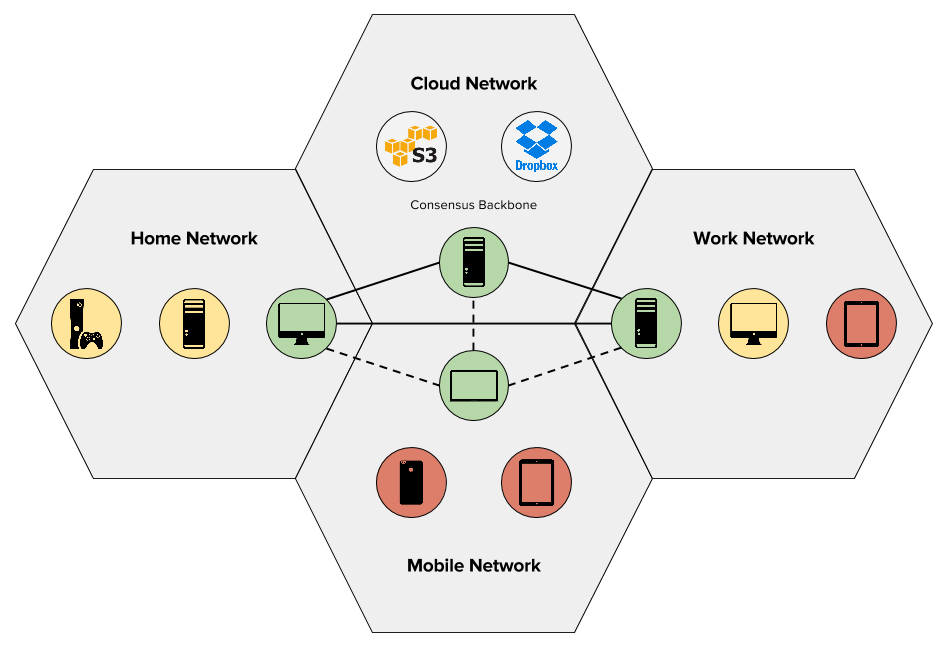
\includegraphics[width=0.5\textwidth]{figures/topology}
    \caption{The topology of a federated consistency model.}
    \label{fig:topology}
\end{figure}

The integration of multiple consistency requires a strong consensus core in order to provide guarantees and manage conflicts, a scheme also used in Oceanstore \cite{kubiatowicz_oceanstore_2000} and further specified by Gray et al. \cite{gray_dangers_1996}. As shown in Figure \ref{fig:topology} a personal cloud can then attach devices of variable consistency levels to communicate with the strong consensus group. In this case, we have represented the consensus group coordinating across the wide area. In this scenario, mobile devices will always have access to a prime replica participating in consensus. Other topologies might include hierarchies of strong consensus groups for both local coordination and wide area synchronization.

\subsection{Interaction at Consistency Boundaries}

For replicas that participate at the same consistency level, their interactions are well specified by the parameters of the implementation of that consistency. However, it must be noted that all replicas have equal opportunity of communication with any other replica that might be participating in the federated system at a different consistency level. Communication between a replica of one consistency level to another is said to be communicating across a \textit{consistency boundary}. Both participants must decide whether or not the communication is valid and how to proceed.

For the purpose of this section, we will describe three consistency levels: \textbf{strong} consistency refers to sequential consistency guaranteed by a consensus protocol, \textbf{causal} refers to a consistency level that tracks dependencies and provides convergence semantics (often called causal+), and \textbf{eventual} refers to a last-writer wins approach to consistency where replication is handled by anti-entropy.

All accesses (reads or writes) by the user are local. Remote reads and writes are caused by the specifics of the consistency level and replication mechanism. E.g. we do not specify that a user can make a remote read or write, but rather that remote reads and writes are part of synchronization. We describe interactions at the consistency boundaries as follows.

\subsubsection{Strong-Eventual}

Strong consistency allows reads of the latest local committed version (read committed) and as a result the possibility of a stale read exists. Eventual consistency allows the read of the latest local version, and so too is also susceptible to stale reads. Neither of these consistency models requires a remote read in order to complete.

A write from an eventual replica to a strong replica appears to the strong replica as though a client were performing a remote write. On the anti-entropy delay, if the eventual replica selects a strong node, then the cached writes are sent to the strong node that checks whether the writes can be applied via a version timestamp. If they can be applied, then they are committed through consensus and acknowledged. The eventual node does not have to wait for the conclusion of the consensus decision, and can simply continue. If the versions cannot be applied, the anti-entropy mechanism will allow the strong node to write the most recent committed versions back to the eventual node.

\subsubsection{Strong-Causal}

Because strong consistency provides sequential ordering, it is by definition providing causal ordering, e.g. if a write happens-before another, it will appear in that order in the log of the strong node. However, in order to allow a causal node to remote read from a strong node, it must first confirm that it has all writes that happened-before that read and merge with the strong node. To optimize this operation, strong nodes can contain per-object dependency information, either session based or explicit, depending on the application.

Similarly, writes from a causal node to a strong node must contain dependency information. If the strong nodes do not have dependent writes, or if the writes on the strong node are ahead of the causal node (a fork has occurred), then the causal node must either converge with the consensus group (e.g. repair its snapshot with the one in the strong group) or issue a series of \textit{new} writes to the consensus group that return the system to a correct state. From the perspective of the causal nodes, this will simply be convergence, from the perspective of the consensus group this will look like a series of completely new operations.

\subsubsection{Eventual-Causal}

In order for an eventual node to interact with causal nodes, it must keep track of dependency information, the simplest form of which is that there are no dependencies on the writes. During anti-entropy the causal nodes are responsible for ensuring that the causal dependencies are maintained. For a remote read from a causal node to an eventual node, it can only read the latest version on the eventual node for which the causal node has all the writes (or that the eventual node can supply during the read). This means that a causal node can only read the latest version to which all writes exist.

For remote writes, during anti-entropy the causal node must also ensure that it has all the dependent writes from the eventual node. If one eventual node does not supply all the dependent writes, then the causal node marks the write as ``pending''. When another anti-entropy session occurs that contribute the missing versions, then the causal node can mark the write as accepted and provide it during local reads.

\subsection{Architecture}

\begin{figure}[h]
    \centering
    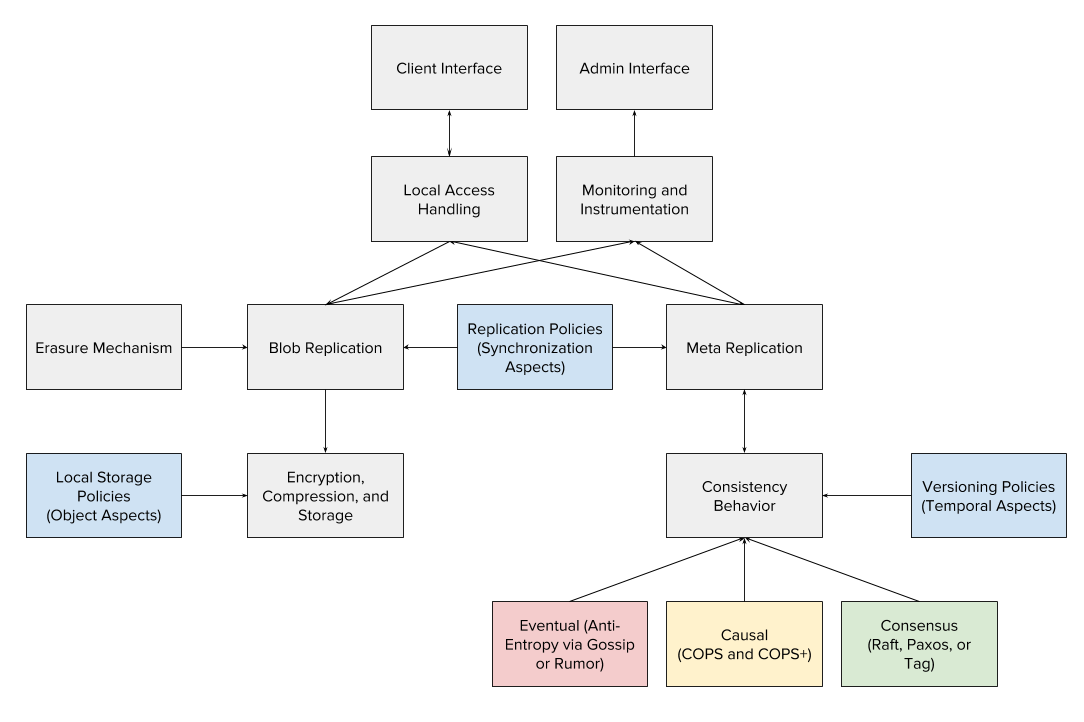
\includegraphics[width=0.5\textwidth]{figures/architecture}
    \caption{The component architecture of a federated consistency model.}
    \label{fig:architecture}
\end{figure}

An architecture for a federated consistency model is specified in Figure \ref{fig:architecture}. In order to optimize federated consistency, we decouple the distribution of object blobs (containing chunks of the the actual data for each version of the object) with decisions concerning the meta data of the system. Blob replication is handled using object aspects: that is what file types and how much data can be stored on a local replica. Blobs are propagated either via direct remote read on access or via anti-entropy mechanisms.

Meta data about the objects in the system, including their key (name), version, consistency level, origin, etc. provide the visibility of the system, and it is this data that must be made consistent across the entire distributed system. As such federated consistency approaches will be applied at this level. Temporal and synchronization policies will govern how meta data is replicated across the system.

\section{Experimental Discussion}

In order to show the need for federated consistency, we have developed a discrete event simulation that implements accesses in a variety of network environments. In particular, we have studied how variable latency affects both eventual and Raft consensus. Figure \ref{fig:ae_stale_reads} and Figure \ref{fig:ae_viz_latency} show how eventually consistent systems are affected by higher latencies with different anti-entropy delays. Figure \ref{fig:ae_viz_ratio} shows how the ratio of fully visible writes to all writes decreases as the latency increases in an eventually consistent system. What this means is that eventual consistency on its own degrades rapidly as the latency increases.

\begin{figure}[h]
    \centering
    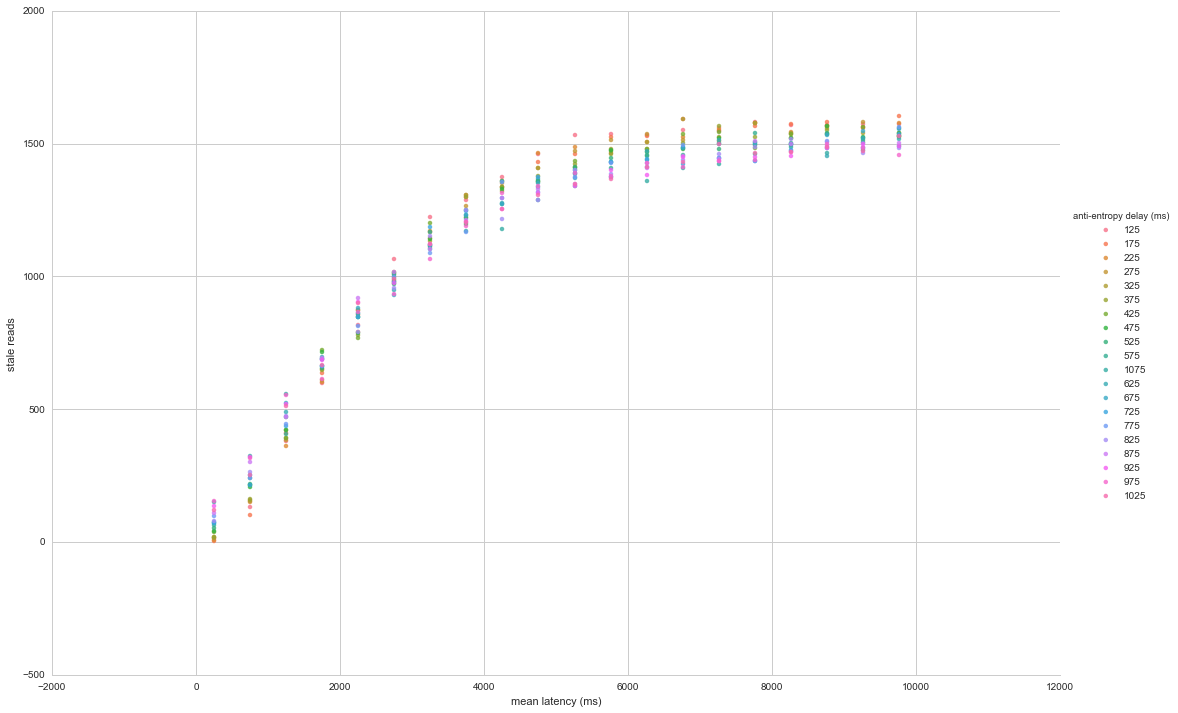
\includegraphics[width=0.5\textwidth]{figures/ae_stale_reads}
    \caption{Stale reads using eventual consistency with variable anti entropy delay.}
    \label{fig:ae_stale_reads}
\end{figure}

\begin{figure}[h]
    \centering
    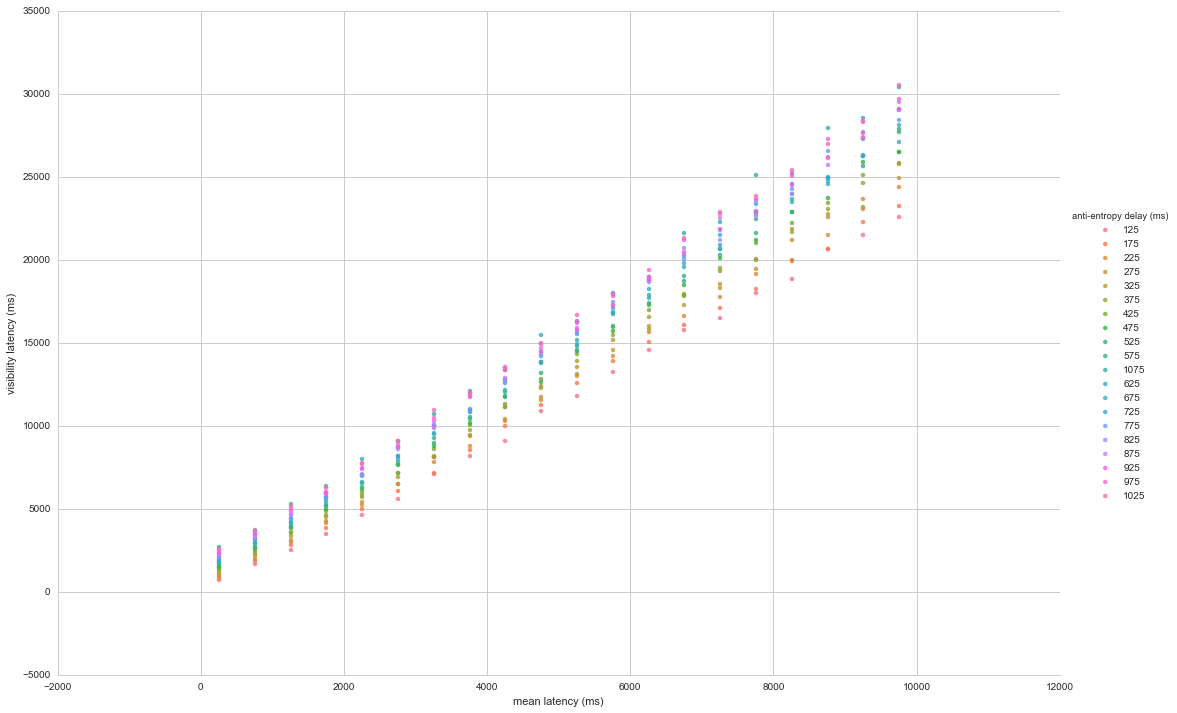
\includegraphics[width=0.5\textwidth]{figures/ae_viz_latency}
    \caption{Visibility latency using eventual consistency with variable anti entropy delay.}
    \label{fig:ae_viz_latency}
\end{figure}

\begin{figure}[h]
    \centering
    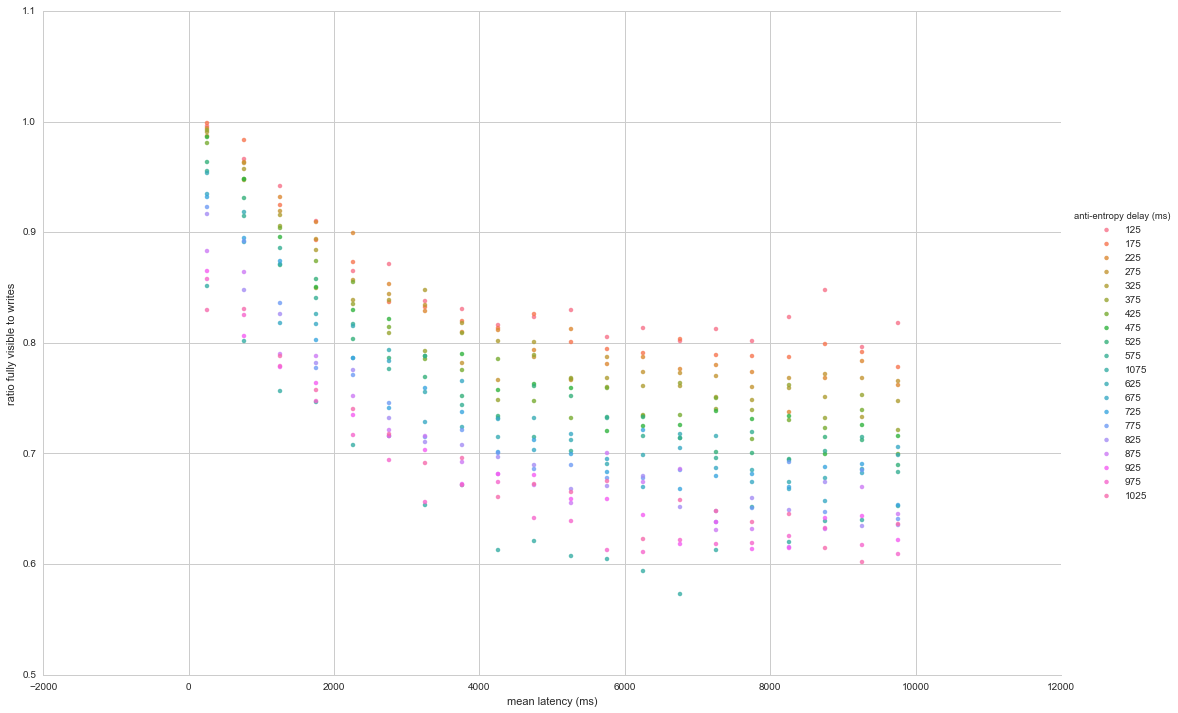
\includegraphics[width=0.5\textwidth]{figures/ae_viz_ratio}
    \caption{Ratio of fully visible writes to total writes using eventual consistency with variable anti entropy delay.}
    \label{fig:ae_viz_ratio}
\end{figure}

In the second part of our experimental results, we study how Raft, an understandable consensus algorithm operates in the network environment we have proposed. In Figure \ref{fig:raft_commit_latency} we show that as the number of users increases, the latency for each commit becomes worse and worse as the mean latency of the system increases. In Figure \ref{fig:raft_latencies} we show how susceptible Raft is to the mean network latency through the various mechanisms of determining the intervals.

\begin{figure}[h]
    \centering
    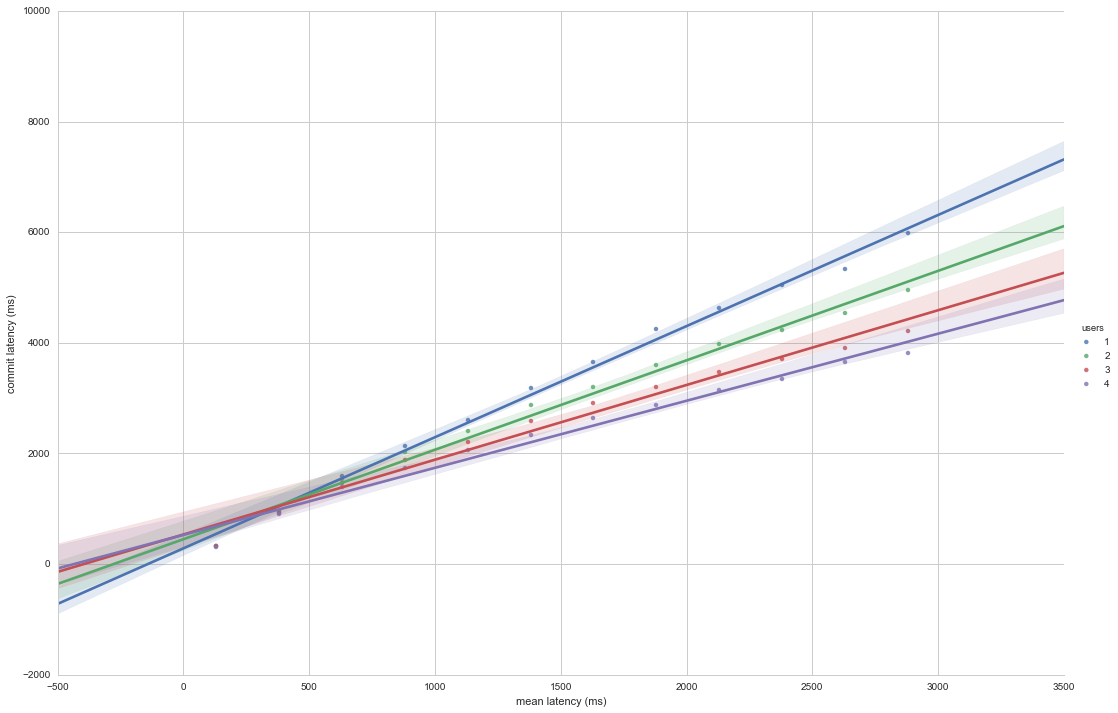
\includegraphics[width=0.5\textwidth]{figures/raft_commit_latency}
    \caption{Commit latency in Raft with increasing numbers of users.}
    \label{fig:raft_commit_latency}
\end{figure}

\begin{figure}[h]
    \centering
    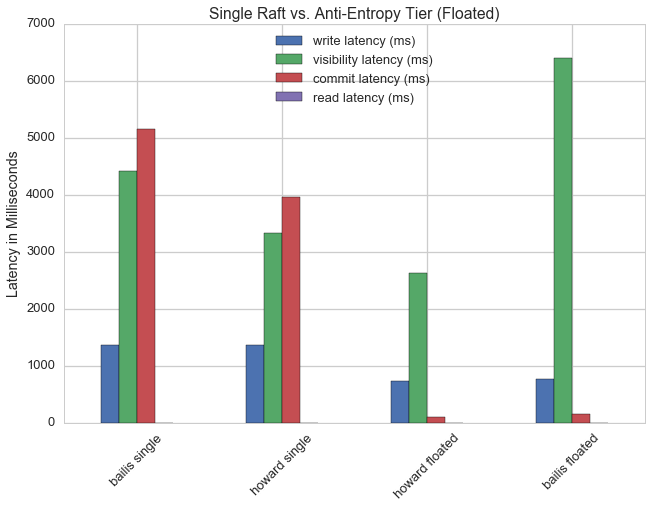
\includegraphics[width=0.5\textwidth]{figures/raft_latencies}
    \caption{Commit latency in Raft for various network parameters implementations.}
    \label{fig:raft_latencies}
\end{figure}

These results are meant to show that federated consistency can take advantage of a number of strong features of consistency models while minimizing their weaknesses particularly in the environments we are talking about.

\section{Conclusion}


\section*{Acknowledgments}

{\footnotesize \bibliographystyle{acm}
\bibliography{references}}

% uncomment to include end notes.
% \theendnotes

\end{document}
